\documentclass[a4paper,twoside,11pt]{article}
\usepackage{a4wide,graphicx,fancyhdr,amsmath,amssymb, enumerate, caption, subcaption, wrapfig}

%----------------------- Macros and Definitions --------------------------

\setlength\headheight{20pt}
\addtolength\topmargin{-10pt}
\addtolength\footskip{20pt}

\newcommand{\HRule}{\rule{\linewidth}{0.5mm}} % Defines a new command for the horizontal lines,
\newcommand{\N}{\mathbb{N}}
\newcommand{\ch}{\mathcal{CH}}

\fancypagestyle{plain}
\fancyhf{}
\fancyhead[LO,RE]{\sffamily\bfseries\large Technische Universiteit Eindhoven}
\fancyhead[RO,LE]{\sffamily\bfseries\large 2IV35 Visualization}
\fancyfoot[LO,RE]{\sffamily\bfseries\large Department of Mathematics and Computer Science}
\fancyfoot[RO,LE]{\sffamily\bfseries\thepage}
\renewcommand{\headrulewidth}{0pt}
\renewcommand{\footrulewidth}{0pt}


\pagestyle{fancy}
\fancyhf{}
\fancyhead[RO,LE]{\sffamily\bfseries\large Technische Universiteit Eindhoven}
\fancyhead[LO,RE]{\sffamily\bfseries\large 2IV35 Visualization}
\fancyfoot[LO,RE]{\sffamily\bfseries\large Department of Mathematics and Computer Science}
\fancyfoot[RO,LE]{\sffamily\bfseries\thepage}
\renewcommand{\headrulewidth}{1pt}
\renewcommand{\footrulewidth}{0pt}


\begin{document}
\begin{titlepage}

\center % Center everything on the page

\textsc{\Huge \textbf{Technische Universiteit Eindhoven}}\\[1.5cm] % Name of your university/college
\textsc{\LARGE \textbf{Visualization}}\\[0.5cm] % Major heading such as course name
\textsc{\large 2IV35}\\[0.5cm] % Minor heading such as course title

\HRule \\[0.4cm]
{ \huge \bfseries Volume rendering}\\[0.4cm] % Title of your document
\HRule \\[1.5cm]

\begin{minipage}{0.4\textwidth}
\begin{flushleft} \large
\emph{\textbf{Author:}}\\
Sander Kools \\
0848523 \\
s.w.a.kools@student.tue.nl % Your name
\end{flushleft}
\end{minipage}
~
\begin{minipage}{0.4\textwidth}
\begin{flushright} \large
\emph{\textbf{Author:}}\\
Luuk Hulten\\
0720248 \\
l.a.j.v.hulten@student.tue.nl
\end{flushright}
\end{minipage}\\[4cm]

{\large \today}\\[3cm] % Date, change the \today to a set date if you want to be precise

\vfill % Fill the rest of the page with whitespace

\end{titlepage}

\newpage
\tableofcontents
\newpage

\section*{Introduction}
In this report we will describe some implementation details of the volume rendering application. We will show the advantages and disadvantages of some rendering techniques at the hand of images and explanations.
In section 1, we will give some details about rendering in a lower resolution to speed up interacting with the application. \newline
In section 2, we will discuss the Compositing rendering technique.
In section 3, we will discuss the Opacity Weighting rendering technique.
In section 4, we will discuss the Trilinear Interpolation technique used.
In section 5, we will discuss the MIP (Maximum Intensity Projection) rendering technique. \newline

\section{Speeding up interaction}
Since most visualization techniques are quite slow, interacting with the visualization becomes laggy and difficult. To speed up these interaction we render the image while interacting in a lower resolution. We implemented the rendering to render the image in three different resolutions. These resolutions are $\frac{1}{4}$ and $\frac{1}{2}$ of the original resolution. At last we render the image at full resolution.

\begin{figure}[h!]
\begin{center}
        \begin{subfigure}[b]{0.3\textwidth}
                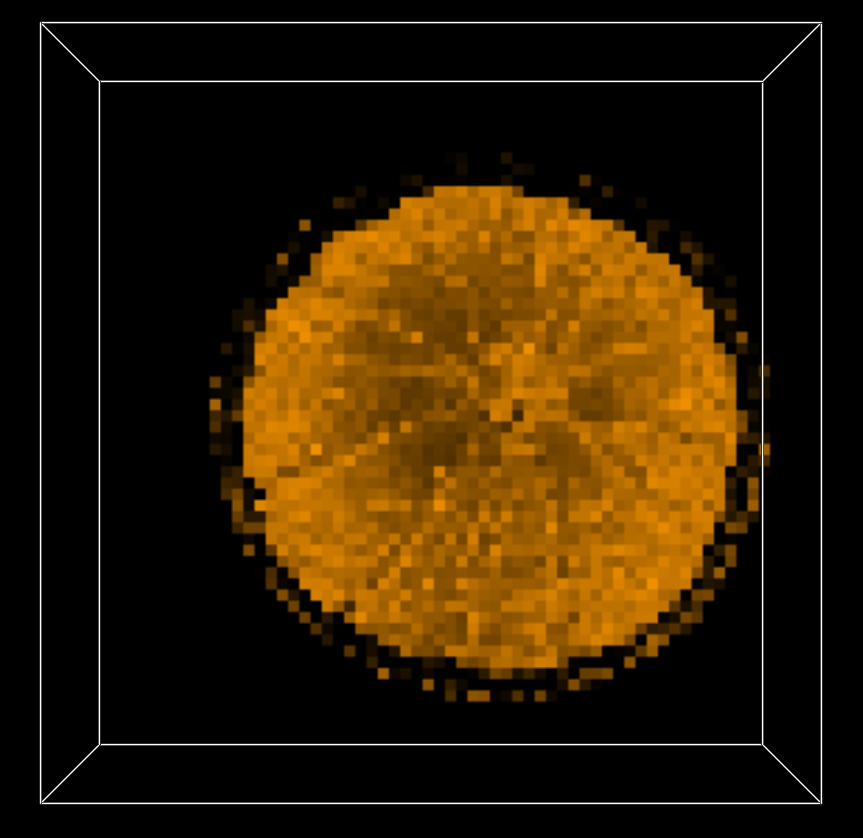
\includegraphics[width=\textwidth]{Images/res4.png}
                \caption{$\frac{1}{4}$ Resolution}
                \label{fig:res4}
        \end{subfigure}
        \begin{subfigure}[b]{0.3\textwidth}
                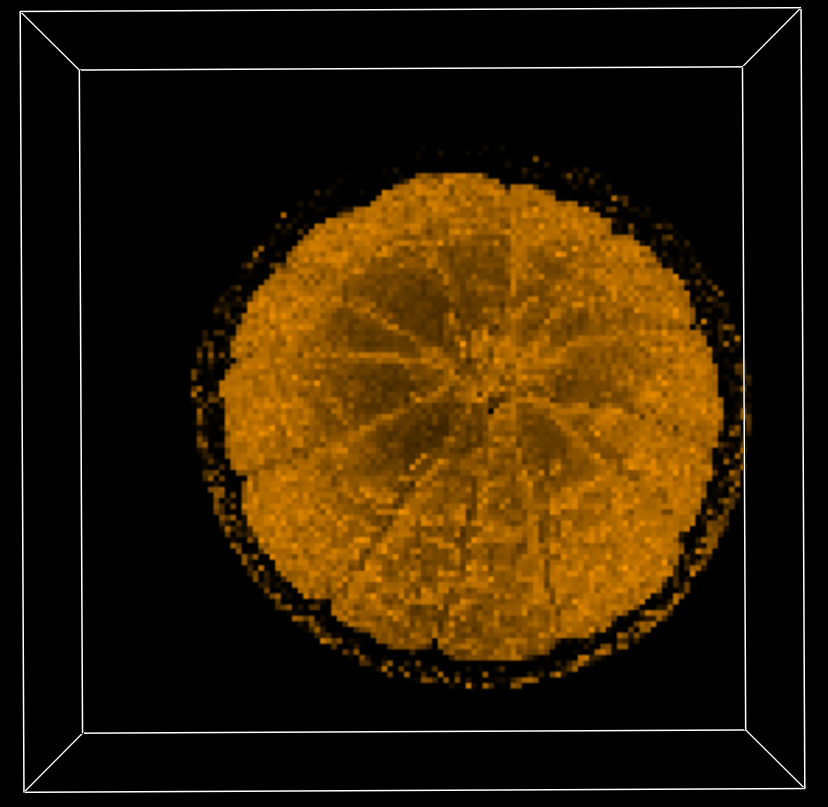
\includegraphics[width=\textwidth]{Images/res2.png}
                \caption{$\frac{1}{2}$ Resolution}
                \label{fig:res2}
        \end{subfigure}
        \begin{subfigure}[b]{0.3\textwidth}
                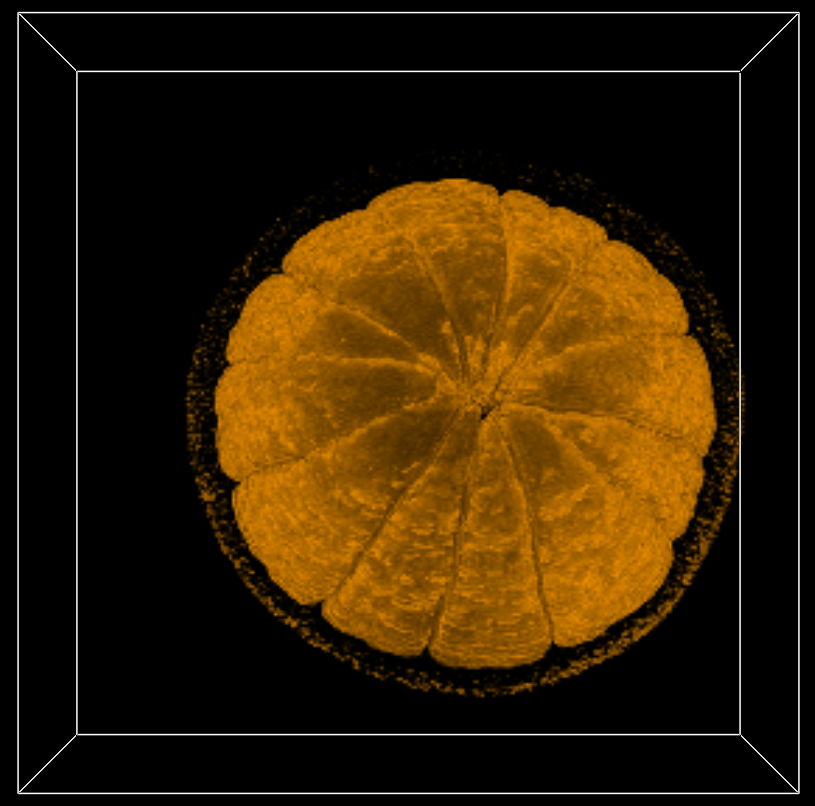
\includegraphics[width=\textwidth]{Images/res1.png}
                \caption{Full resolution}
                \label{fig:res1}
        \end{subfigure}
\end{center}
\end{figure}
\newpage


\section{Compositing}
With compositing the colors along the the ray are combined together using the alpha values of that color. Compositing can be done in two directions depending on the direction the ray is cast.
We used the back to front variant using the following formula:
\begin{equation}\label{Compositing}
  c_i = \sigma_i * c_i + (1 - \sigma_i) * c_{i-1}
\end{equation}
This formula is used for each component (alpha, red, green, blue) of the color.
The following images have been produced using the compositing rendering technique.

\begin{figure}[h!]
    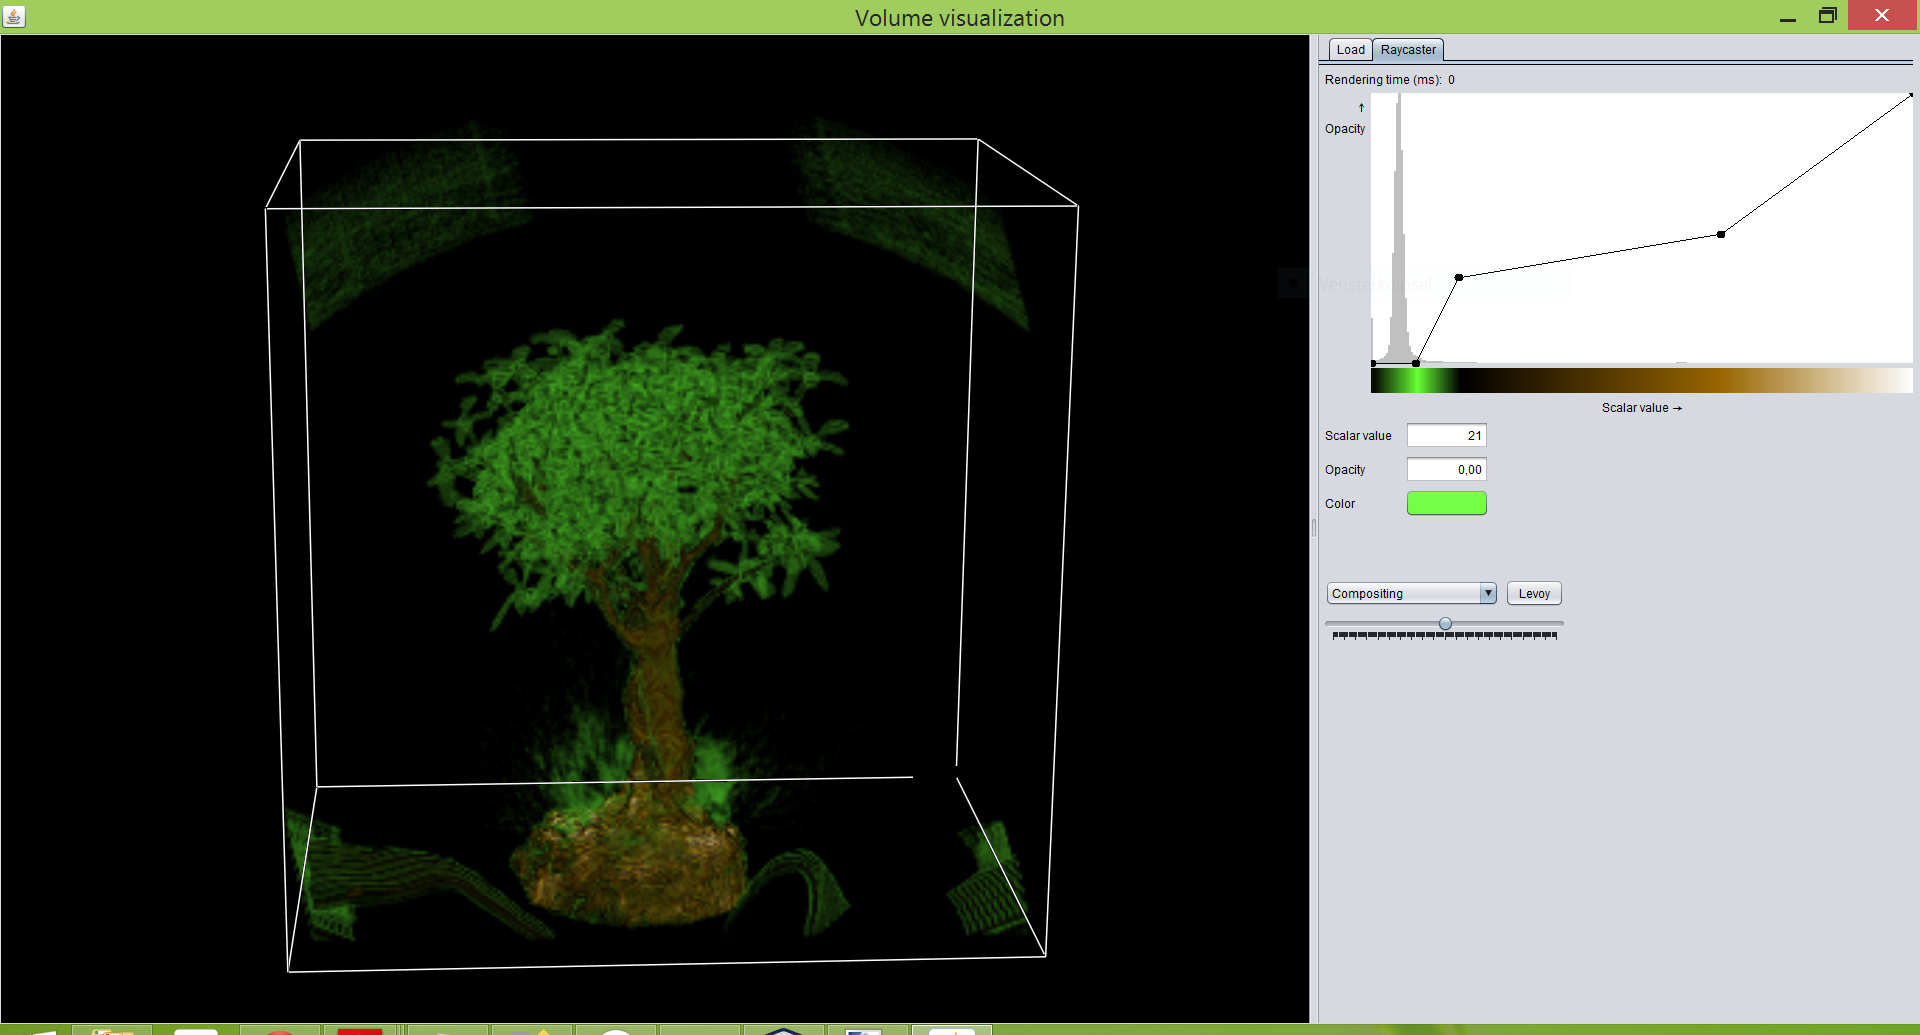
\includegraphics[width=\textwidth]{Images/BonsaiCOMP.png}
    \caption{Bonsai Compositing}
    \label{fig:BonsaiCOMP}
\end{figure}

\begin{figure}[h!]
    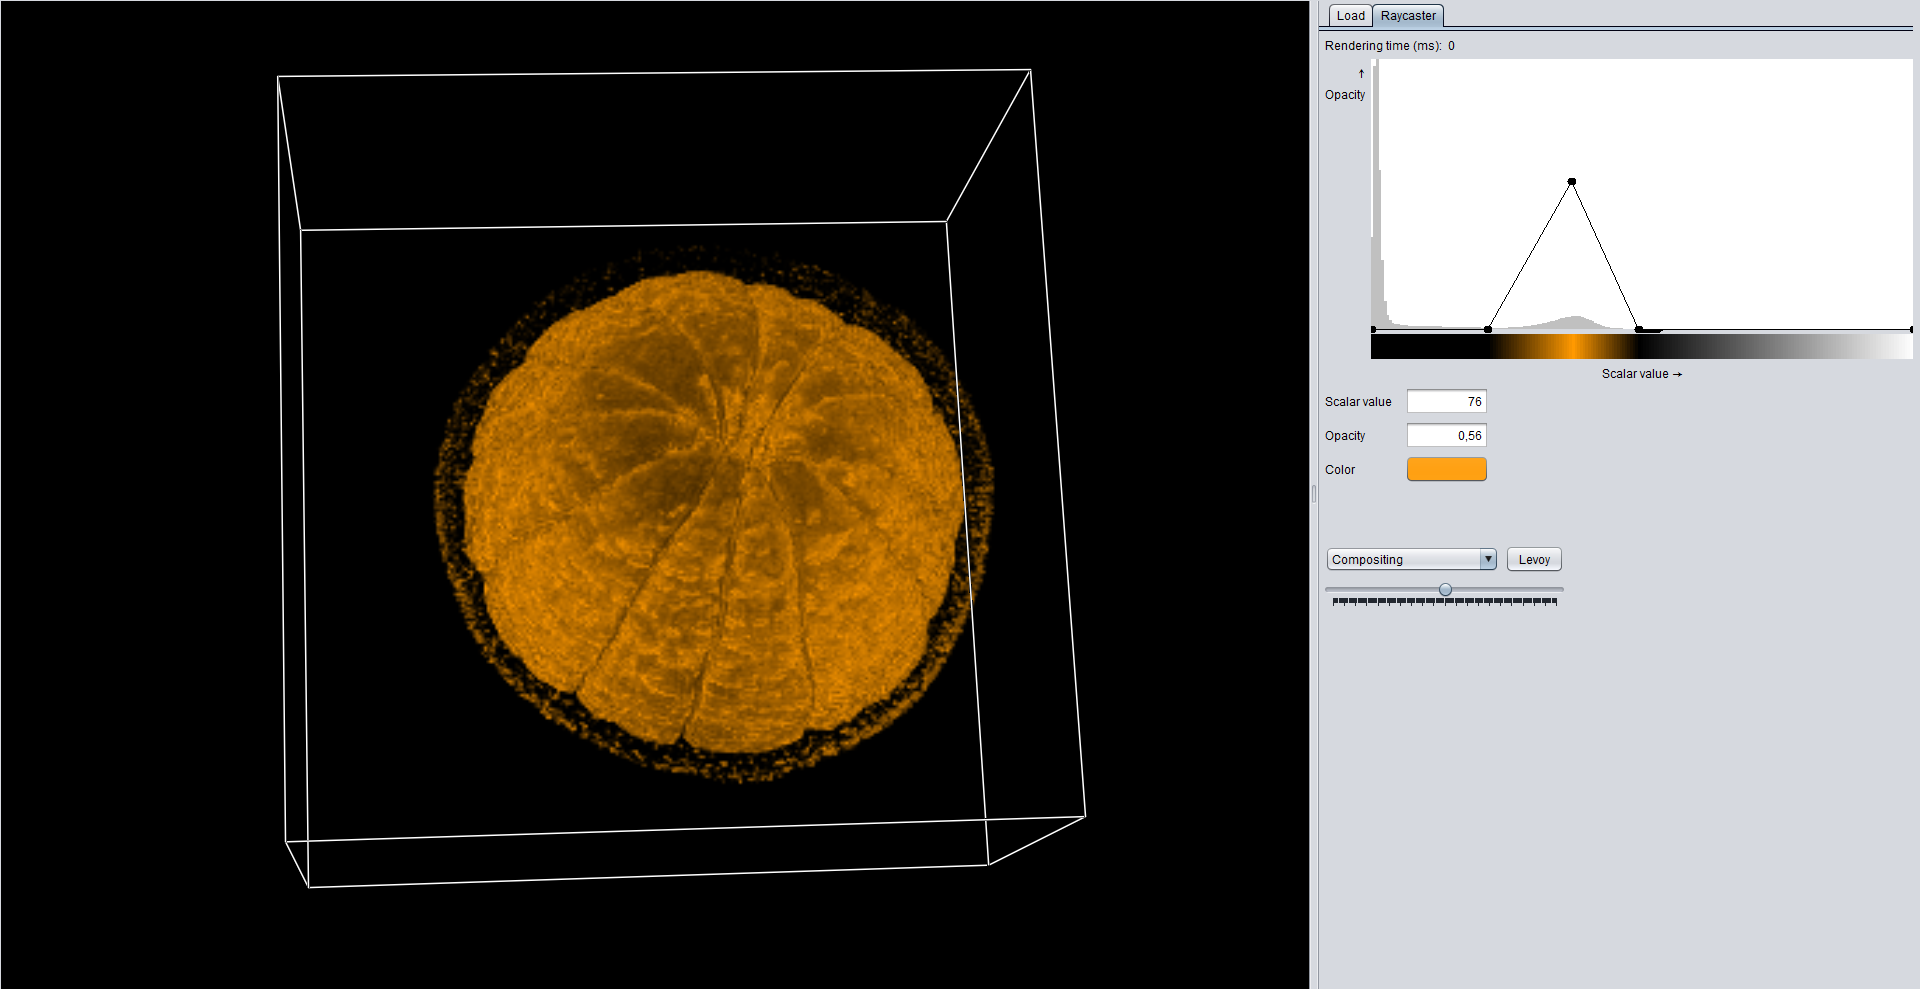
\includegraphics[width=\textwidth]{Images/OrangeCOMP.png}
    \caption{Orange Compositing}
    \label{fig:OrangeCOMP}
\end{figure}

\begin{figure}[h!]
    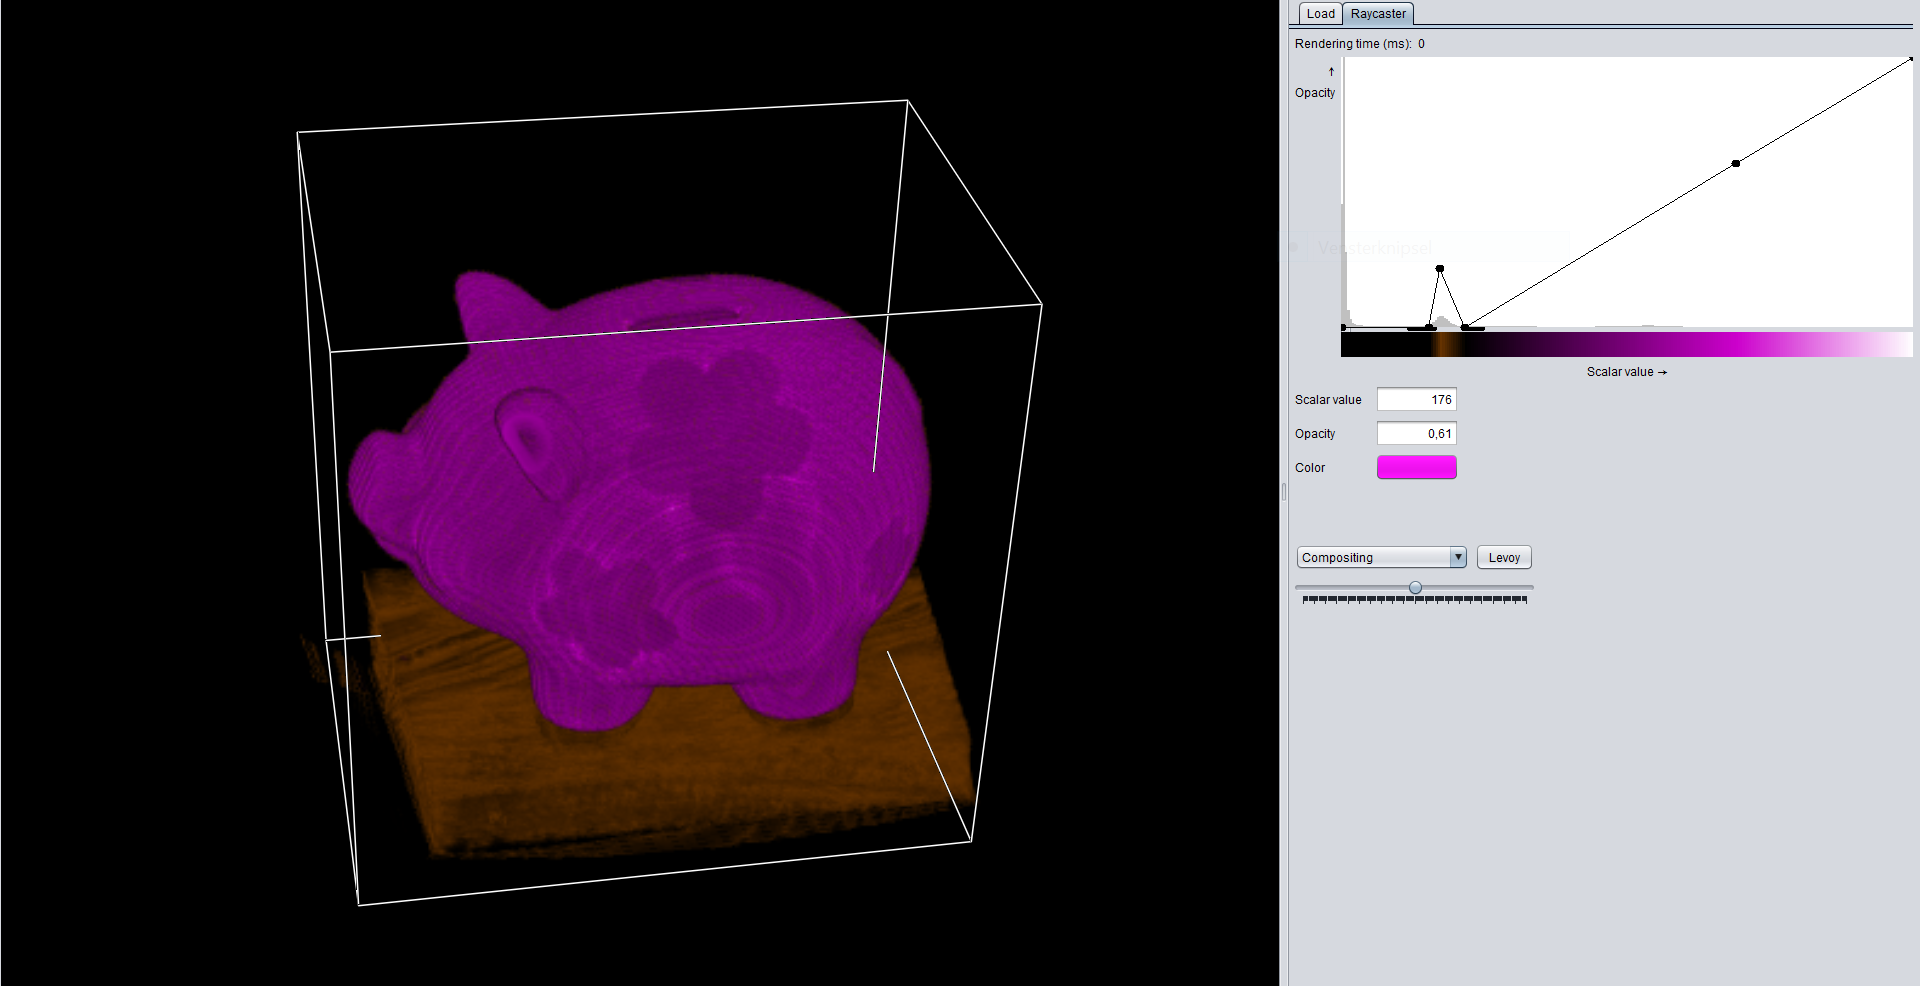
\includegraphics[width=\textwidth]{Images/PigCOMP.png}
    \caption{Pig Compositing}
    \label{fig:PigCOMP}
\end{figure} \newpage

As seen in the previous images compositing delivers more sophisticated images in compare to the MIP rendering technique. This was to be expected since MIP only uses one value along the ray, while compositing uses all the values with respect to its alpha value, combining them to a single color. As seen in the pictures this technique shows more details in the rendered images. \newline
Compositing is best used for rendering the outside of objects from volume data.
\newpage

\section{Opacity Weighting}
Opacity weighting is a rendering technique where opacity are scaled depending on material values selected by the user. With these values a volume of opacities is calculated. In this volume each voxel has a opacity scaled to the selected material values and the local gradient magnitude. After these alpha values have been calculated a ray is cast into this volume and with the compositing technique merged into one color value that is projected on the view plane.
\begin{figure}[h!]
    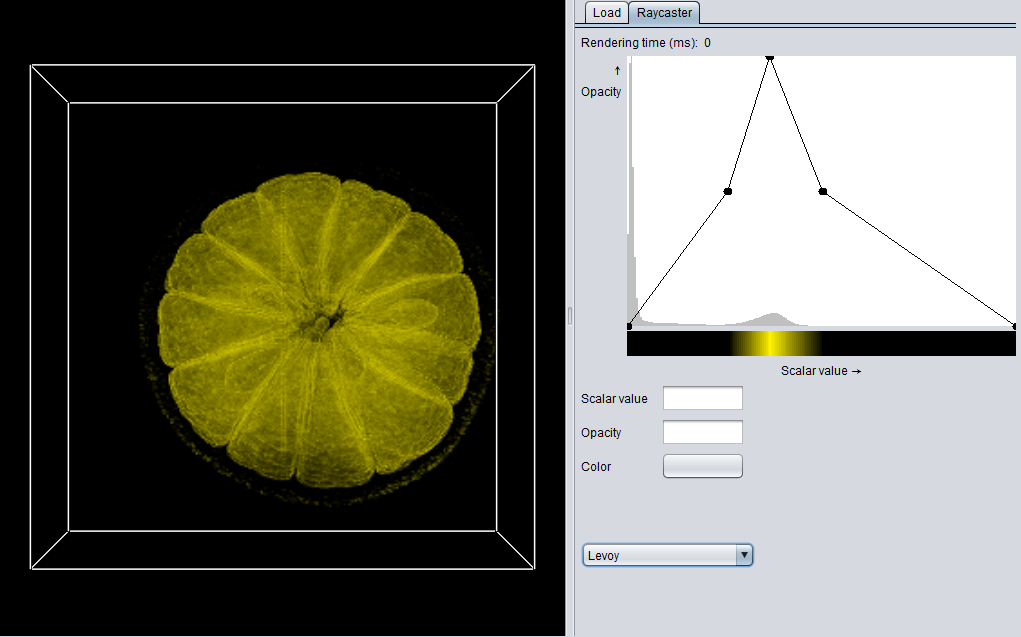
\includegraphics[width=\textwidth]{Images/OrangeOW.png}
    \caption{Orange Opacity Weighting}
    \label{fig:BonsaiOW}
\end{figure}
Calculating these opacity values takes a long time since it has to be done for every voxel. Since these opacity values are independent of the view vector the rendered image can be rotated without having to recalculate all opacity values. However changing the material choice values will result in a full recalculation of all voxel alpha values. We used the transfer function control points to input the values $f_{v_{n}}$ and $a_{v_{n}}$ since this was already implemented and was easy to implement the new functionality. \newpage

As shown in figure \ref{fig:BonsaiOW} and \ref{fig:OrangeOW} images rendered using opacity weighting looks to have no volume. You see through the volume to the other side as it was hollow. This is as expected since the article explains that where selected tissues contact other tissue these voxels get the highest opacities.

\begin{figure}[h!]
\begin{center}
    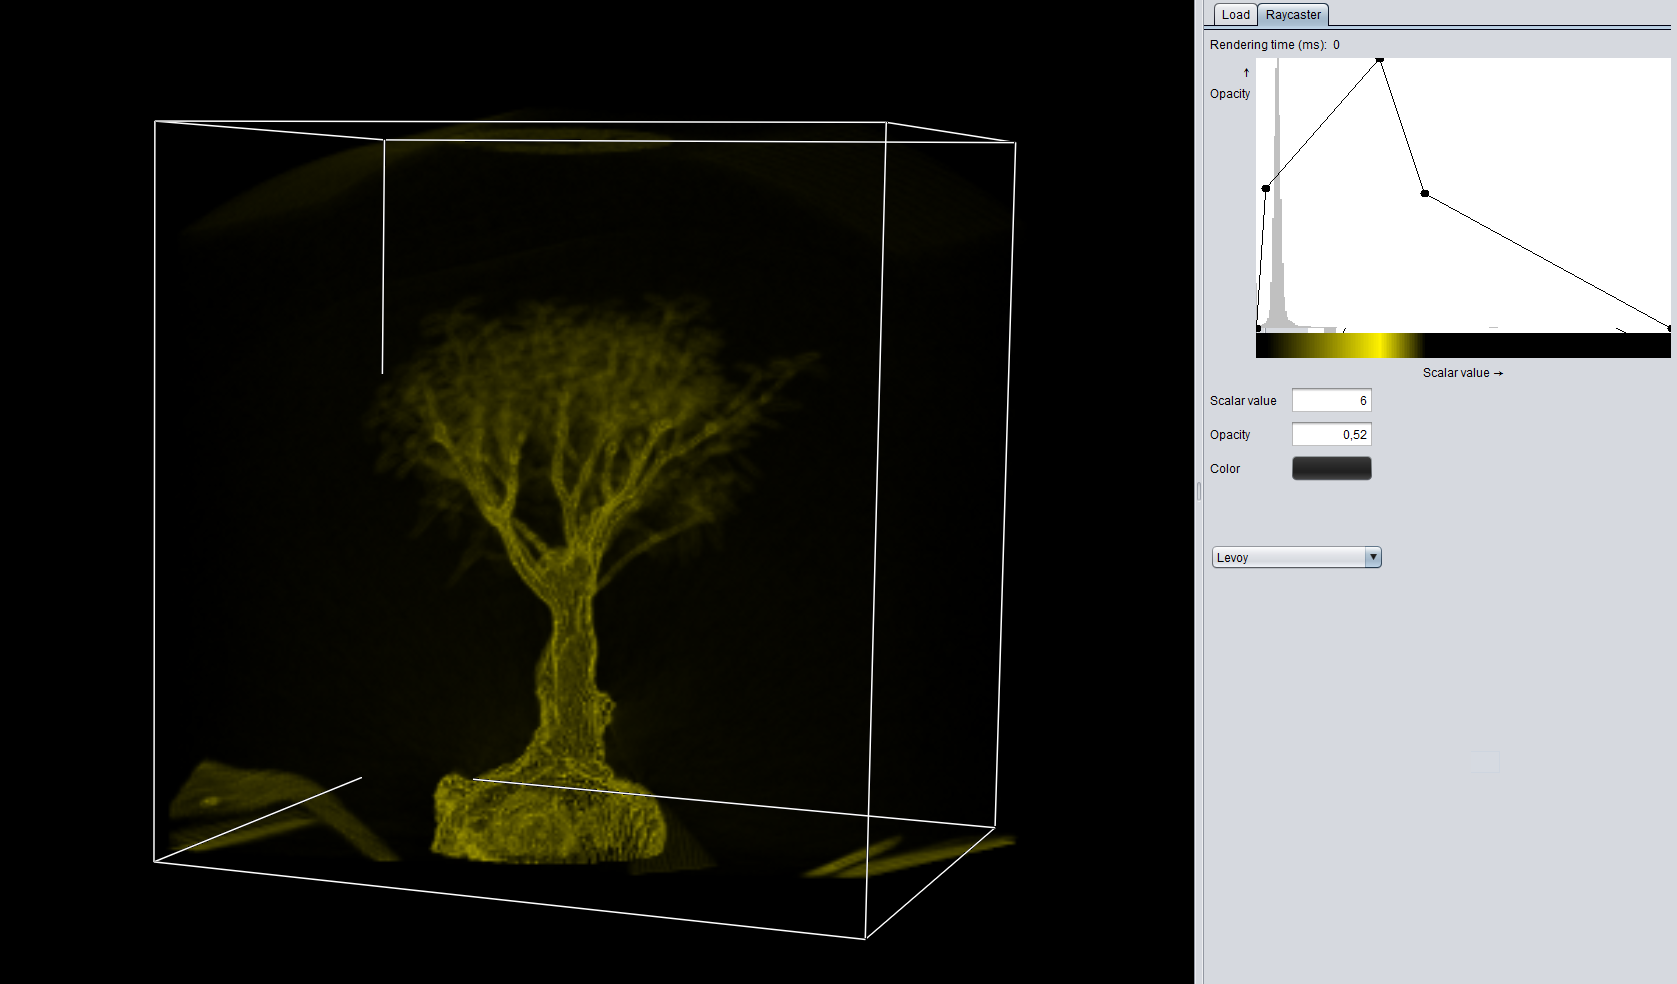
\includegraphics[width=0.7\textwidth]{Images/BonsaiOW.png}
    \caption{Bonsai Opacity Weighting}
    \label{fig:OrangeOW}
\end{center}
\end{figure}
This rendering technique is suitable for identifying and selecting different tissue types in volumetric data without a boolean decision if the tissue is in or out the volume.
\begin{figure}[h!]
\begin{center}
    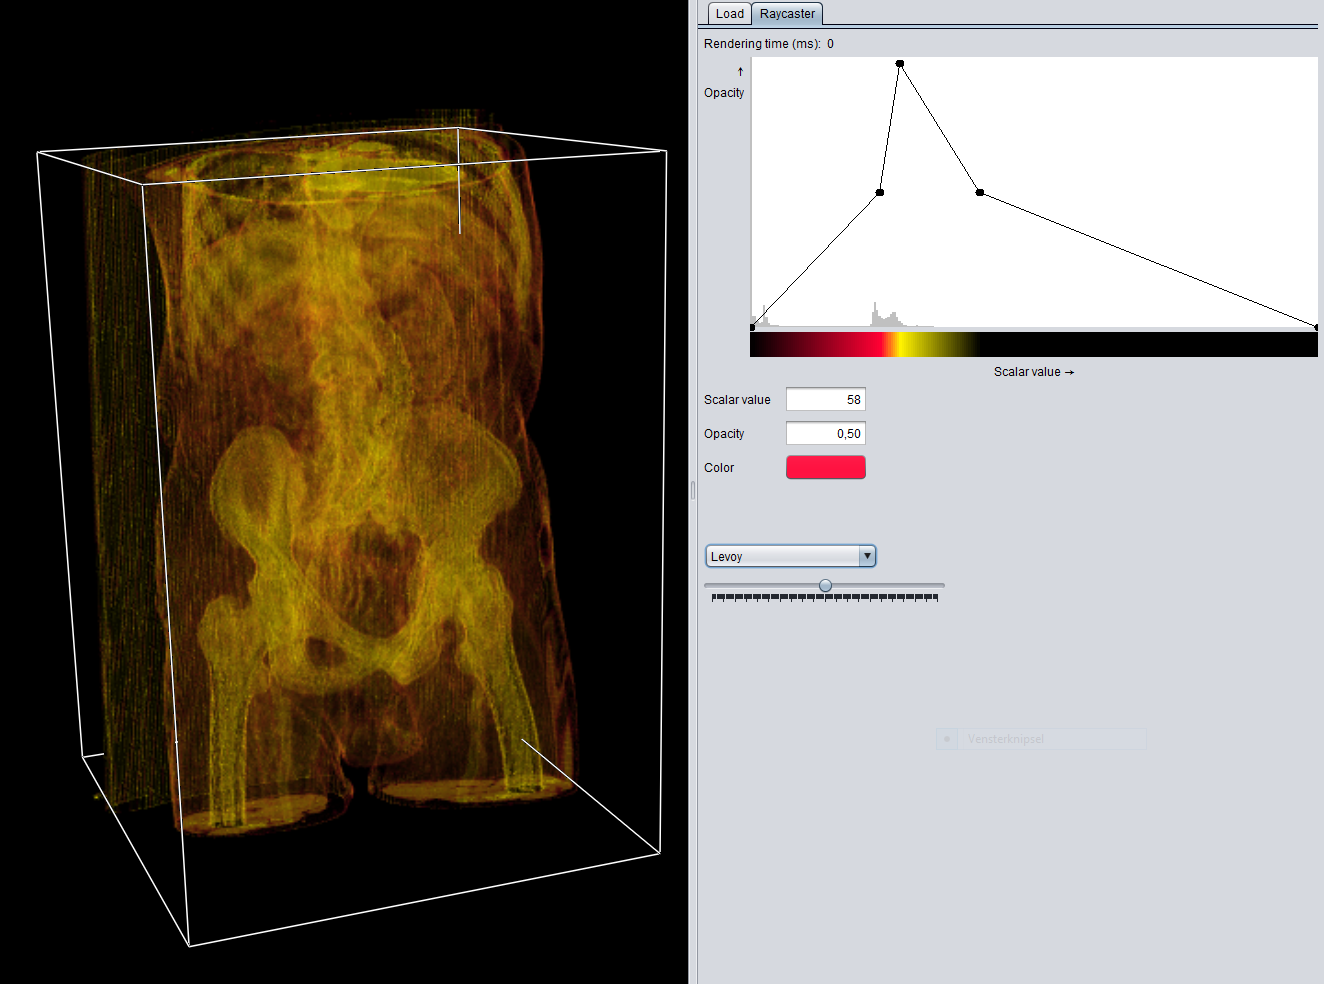
\includegraphics[width=0.7\textwidth]{Images/StentOW.png}
    \caption{Stent Opacity Weighting}
    \label{fig:StentOW}
\end{center}
\end{figure}
\newpage
\section{Trilinear Interpolation}
We also implemented tilinear interpolation, this allows us to be able to get an approximate value of a voxel, which ordinarily might not correspond with the raw data points. \newline
Trilinear interpolation is the extension of linear interpolation and bilinear interpolation and operates in 3 dimensions, in figure \ref{fig:interpolation} you can see an example representation of trilinear interpolation. \newline
Below is the algorithm to compute the point c in figure \ref{fig:interpolation} that we used in the program.
\begin{figure}[h]
    \begin{center}
        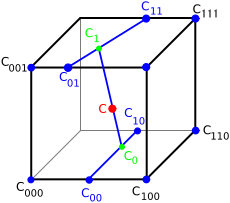
\includegraphics[width=0.4\textwidth]{SanderImages/interpolation.png}
        \caption{representation of trilinear interpolation}
        \label{fig:interpolation}
    \end{center}
\end{figure}
\begin{center}
$x_d = \frac{x-x_0}{x_1-x_0}$ \newline
$y_d = \frac{y-y_0}{y_1-y_0}$ \newline
$z_d = \frac{z-z_0}{z_1-z_0}$ \newline
$c_{00} = V_{x_0,y_0,z_0} \cdot (1-x_d) + V_{x_1,y_0,z_0} \cdot x_d$ \newline
$c_{10} = V_{x_0,y_1,z_0} \cdot (1-x_d) + V_{x_1,y_1,z_0} \cdot x_d$ \newline
$c_{01} = V_{x_0,y_0,z_1} \cdot (1-x_d) + V_{x_1,y_0,z_1} \cdot x_d$ \newline
$c_{11} = V_{x_0,y_1,z_1} \cdot (1-x_d) + V_{x_1,y_1,z_1} \cdot x_d$ \newline
$c_{0} = c_{00} \cdot (1-y_d) + c_{10} \cdot y_d$ \newline
$c_{1} = c_{01} \cdot (1-y_d) + c_{11} \cdot y_d$ \newline
$c = c_{0} \cdot (1-z_d) + c_{1} \cdot z_d$ \newline
\end{center}
\newpage
\section{MIP}
In scientific visualization, a maximum intensity projection (MIP) is a volume rendering method for 3D data. It consists of projecting the voxel with the highest attenuation value on every view throughout the volume onto a 2D image. \newline
This method tends to display bone and contrast material–filled structures preferentially, and other lower-attenuation structures are not well visualized. The primary clinical application of MIP is to improve the detection of pulmonary nodules and assess their profusion. MIP also helps characterize the distribution of small nodules. In addition, MIP sections of variable thickness are excellent for assessing the size and location of vessels, including the pulmonary arteries and veins. \newline
For the implementation of the MIP we sampled every pixel by casting a ray through the data and set the voxel to the maximum value. First we iterate over every pixel. At every pixel we record the corresponding voxel value and if it's the highest value we've encountered, we save it as being the highest value until we possibly find a higher one later in the iteration. \newline
Below in figure \ref{fig:FishMIP} there is an example of a MIP rendering using the fish dataset and the compositing as comparison in figure \ref{fig:FishComp}.
\begin{figure}[h!]
    \begin{center}
        \begin{subfigure}[b]{0.47\textwidth}
            \includegraphics[width=\textwidth]{SanderImages/visMIPZ.png}
            \caption{Fish MIP rendering}
            \label{fig:FishMIP}
        \end{subfigure}
        \begin{subfigure}[b]{0.49\textwidth}
            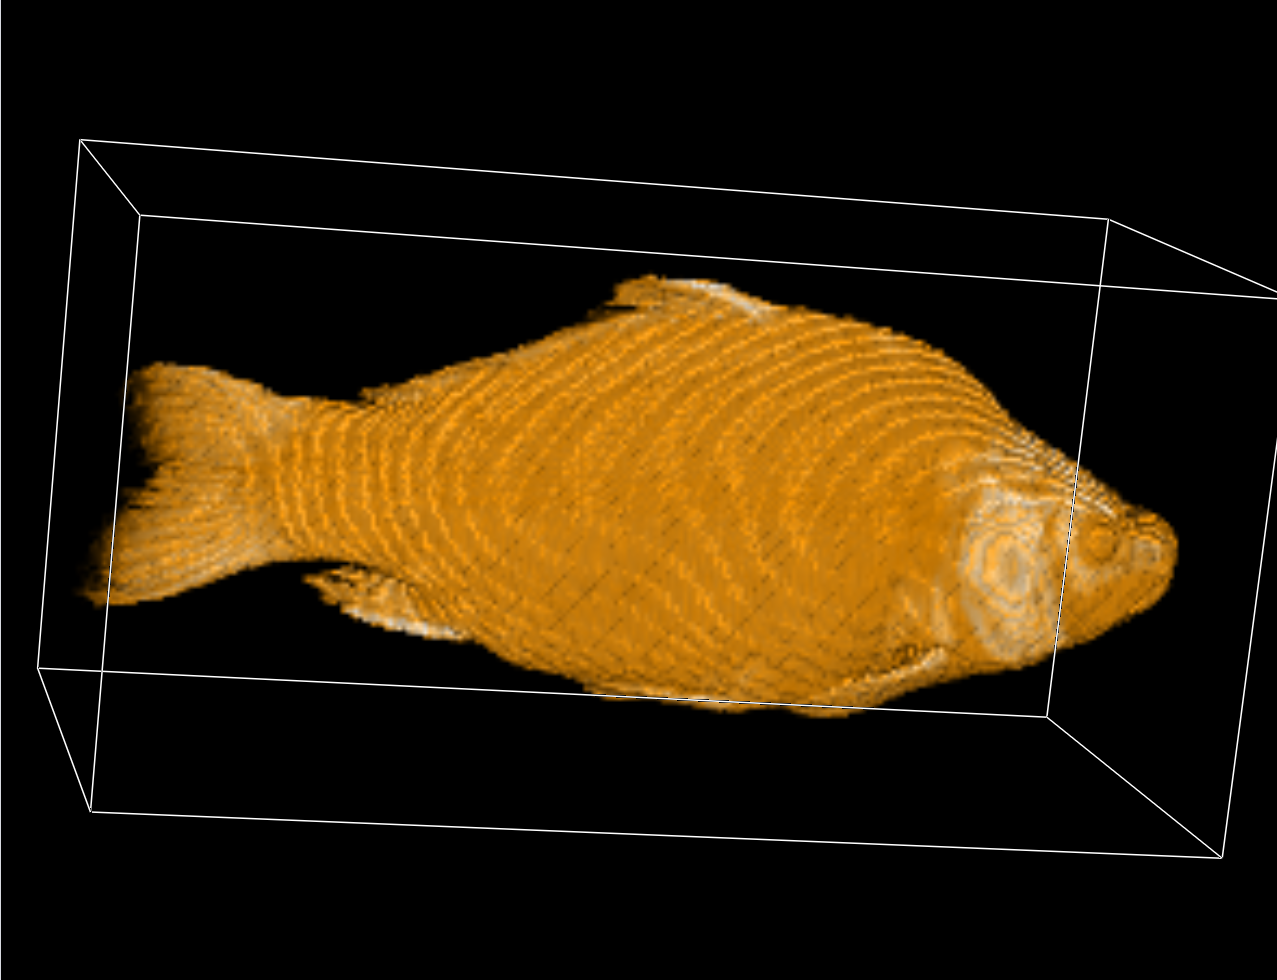
\includegraphics[width=\textwidth]{SanderImages/FishCompZ.png}
            \caption{Fish Compositing rendering}
            \label{fig:FishComp}
        \end{subfigure}
        \caption{Fish rendering, MIP and compositing}
    \end{center}
\end{figure} \newline
We see that MIP works well when the datasets have objects with high density, such as the Fish or the Skeleton, for instance in figure \ref{fig:PigMIP} you are able to see the contents of the Piggy bank using this rendering form, which wasn't able with the compositing rendering.

\newpage

\begin{figure}[h!]
    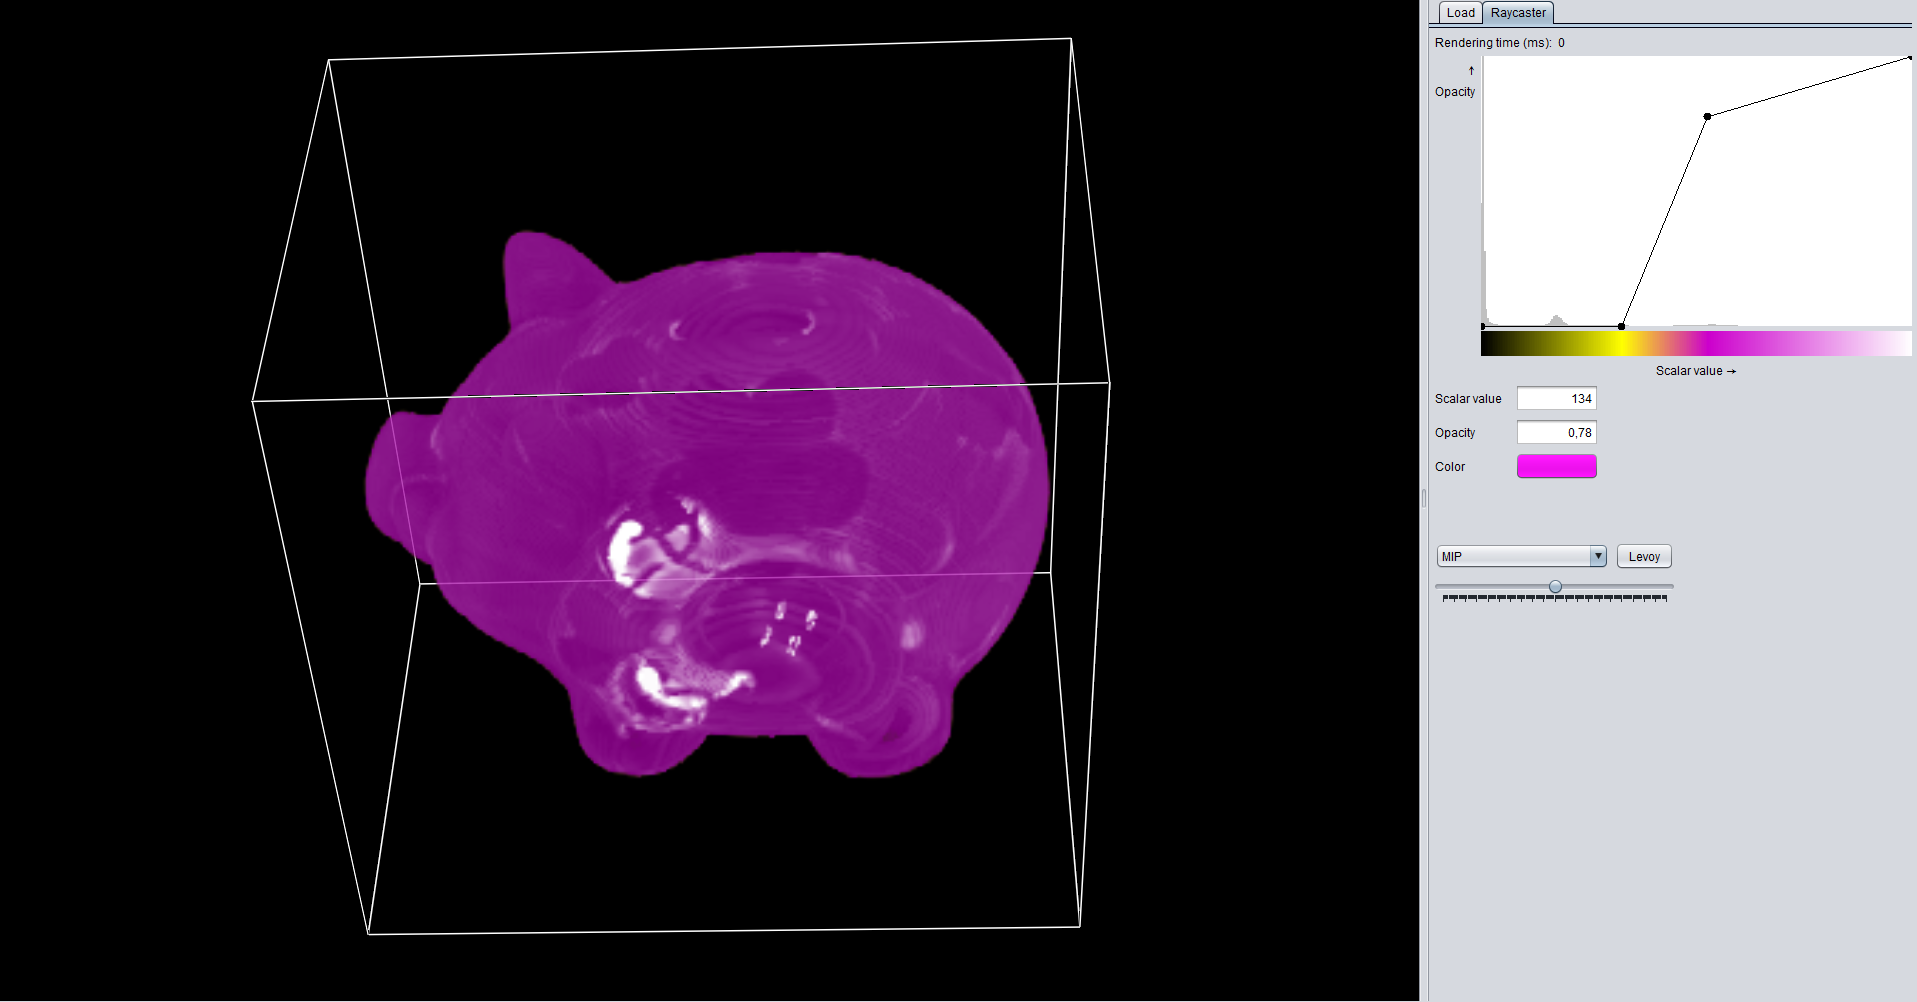
\includegraphics[width=\textwidth]{SanderImages/PigMIP2.png}
    \caption{Pig MIP}
    \label{fig:PigMIP}
\end{figure}

\begin{figure}[h!]
    \begin{center}
        \begin{subfigure}[b]{0.32\textwidth}
            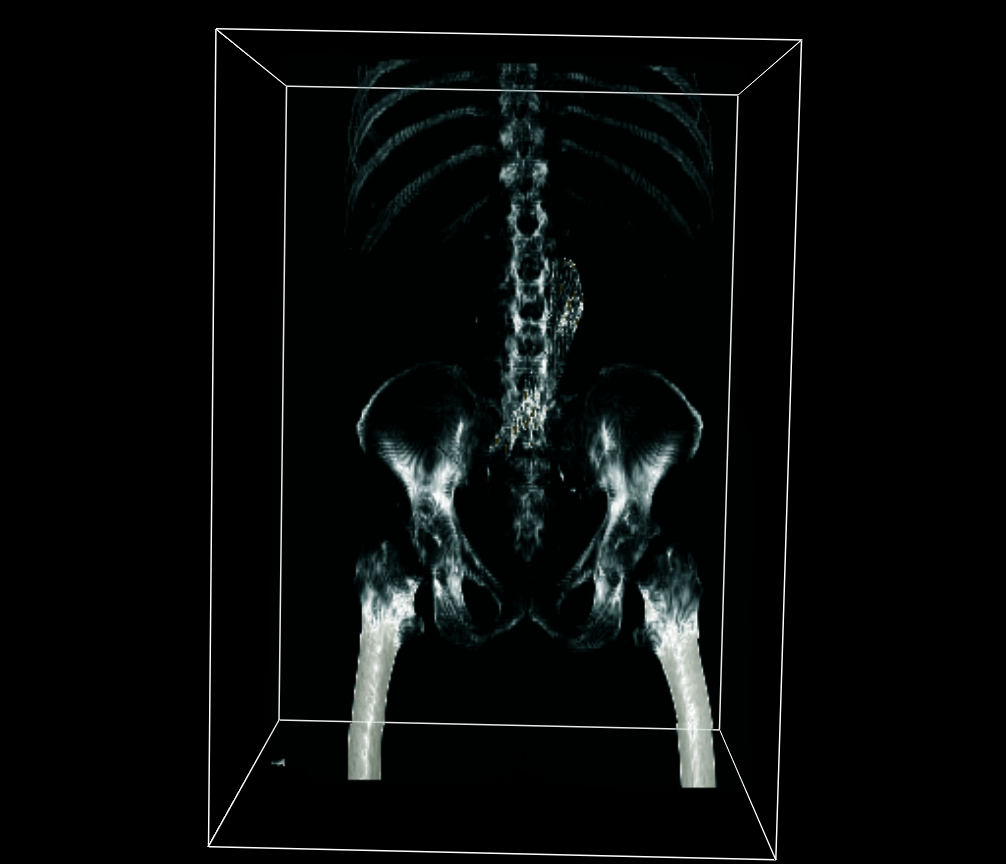
\includegraphics[width=\textwidth]{SanderImages/SkeletonMIPZ.png}
            \caption{Skeleton MIP}
            \label{fig:Skeleton}
        \end{subfigure}
        \begin{subfigure}[b]{0.33\textwidth}
            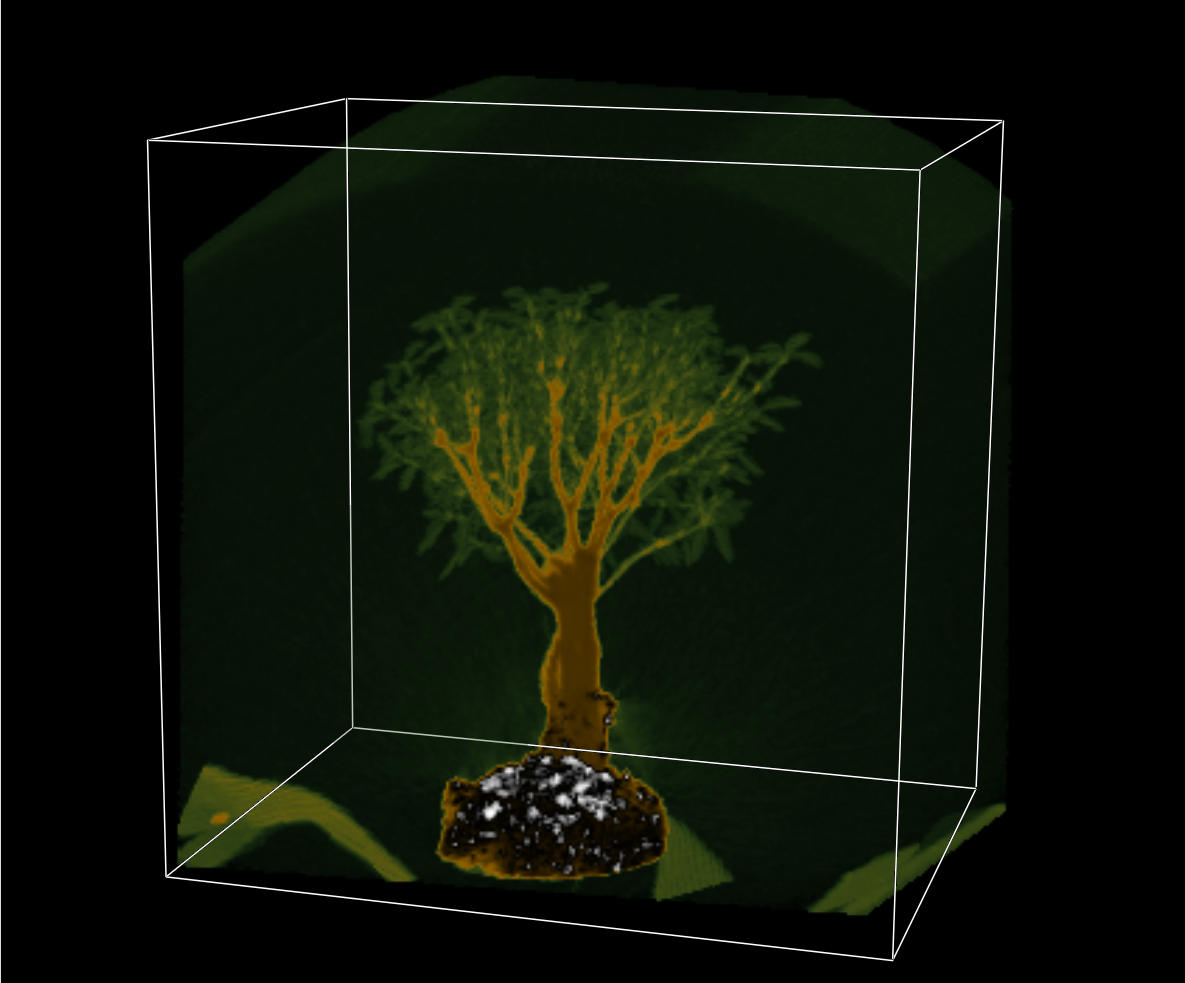
\includegraphics[width=\textwidth]{SanderImages/BonsaiMIPZ.png}
            \caption{Bonsai MIP}
            \label{fig:Bonsai}
        \end{subfigure}
        \begin{subfigure}[b]{0.30\textwidth}
            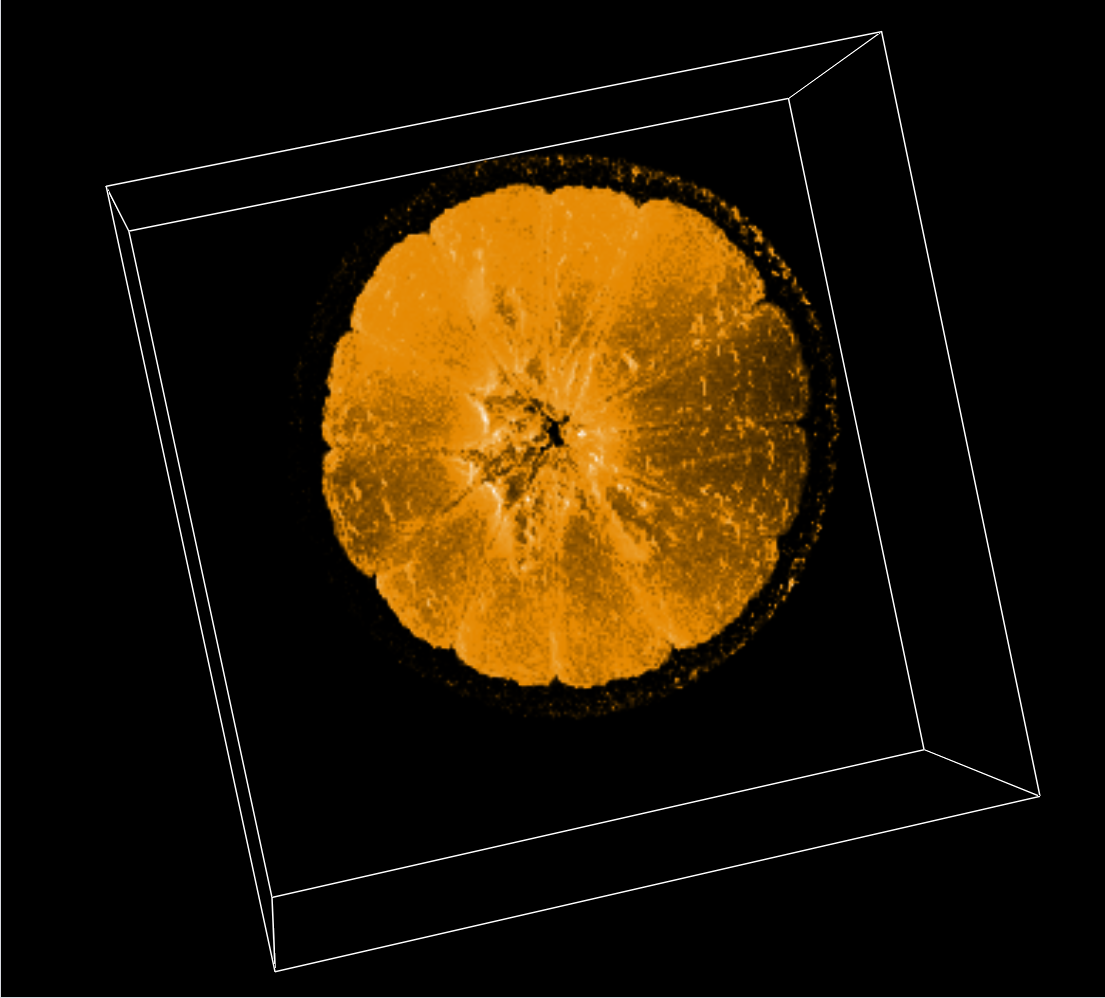
\includegraphics[width=\textwidth]{SanderImages/OrangeMIPZ.png}
            \caption{Orange MIP}
            \label{fig:OrangeMIP}
        \end{subfigure}
        \caption{Multiple MIP renderings}
    \end{center}
\end{figure}
\newpage


\end{document}

